%! Unidad 6 — Campo magnético e inducción electromagnética (teoría, actividades resueltas y prácticas)
%! Fuente: Fuentes/Tema_6.pdf (reescrito; datos de las actividades cambiados y recalculados)

\section*{Para empezar: la aguja que se movió}
\addcontentsline{toc}{section}{Para empezar: la aguja que se movió}

En 1820, durante una clase en Copenhague, Hans Christian Oersted conectó un circuito junto a una brújula y vio cómo la aguja
giraba. Hasta entonces la electricidad y el magnetismo se consideraban fenómenos distintos; aquel pequeño giro demostró que
una corriente eléctrica crea un campo magnético. Once años después, Michael Faraday descubrió el efecto contrario: un campo
magnético que cambia produce una corriente. De esas dos ideas salen los motores, los generadores de las centrales, los
transformadores, los altavoces o las placas de inducción de la cocina. En esta unidad estudiaremos el campo magnético, la
fuerza que ejerce sobre cargas y corrientes, cómo lo crean las corrientes y cómo, al variar, induce corrientes eléctricas.

\section{Imanes y campo magnético}\label{sec:mag-imanes}

El \rojon{magnetismo} es la propiedad de algunos cuerpos, como la magnetita (\ch{Fe3O4}), de atraer el hierro. Los imanes
pueden ser naturales o artificiales (piezas de acero imantadas). Sus propiedades básicas son:
\begin{itemize}
    \item El magnetismo es más intenso en los extremos, los \azuln{polos}. Un imán que puede girar libremente orienta uno de
    ellos hacia el norte geográfico: es su \emph{polo norte}. El otro es el \emph{polo sur}.
    \item Los polos del mismo nombre se repelen y los de distinto nombre se atraen. Por eso el polo norte de una brújula
    señala el norte geográfico: allí está el polo \emph{sur} magnético de la Tierra.
    \item \textbf{No se pueden separar los polos}: si se parte un imán, cada trozo es un imán completo con sus dos polos. No
    existen «cargas magnéticas» aisladas.
\end{itemize}

La región que rodea un imán, en la que se notan sus efectos, es su \rojon{campo magnético}. Es un campo vectorial que se
representa con el vector \azuln{inducción magnética} \(\vec B\) (o, simplemente, campo magnético). Sus líneas de campo salen del
polo norte, entran por el polo sur y continúan por dentro del imán: \textbf{son líneas cerradas}, sin principio ni fin
(figura~\ref{fig:mag-iman}).

\begin{figure}[H]
    \centering
    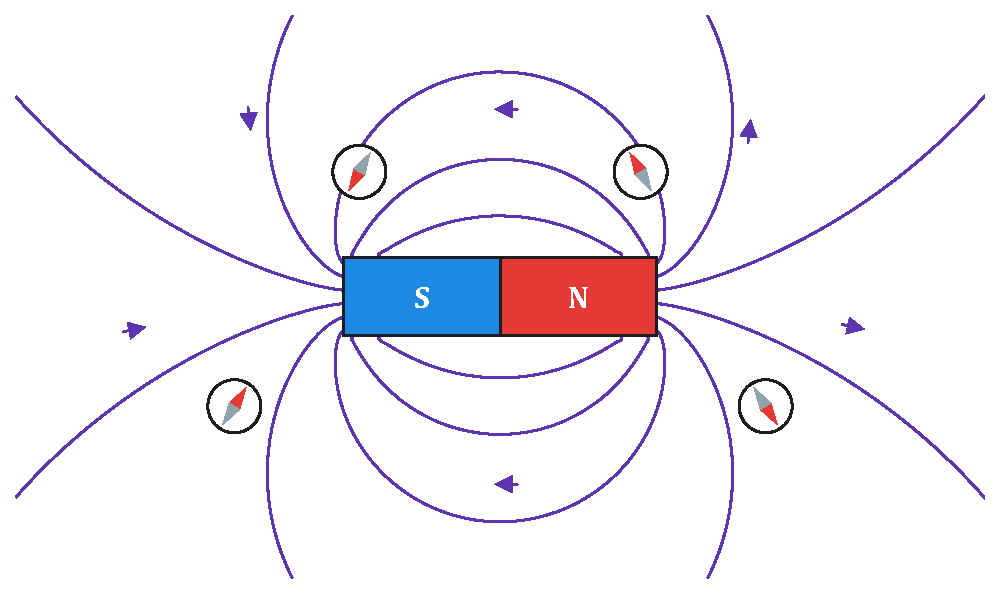
\includegraphics[width=0.7\linewidth]{images/UD6/iman}
    \caption{Líneas del campo de un imán de barra. Las brújulas se orientan tangentes a ellas, con su polo norte (rojo) en el
    sentido del campo.}
    \label{fig:mag-iman}
\end{figure}

\paragraph{Origen del magnetismo natural.} En los átomos, los electrones giran alrededor del núcleo y sobre sí mismos: cada
átomo es un pequeño imán. En la mayoría de los materiales estos imanes elementales están orientados al azar y se anulan. Según
su comportamiento, las sustancias son:
\begin{itemize}
    \item \textbf{Ferromagnéticas} (hierro, cobalto, níquel): son atraídas fuertemente por un imán y se imantan con facilidad.
    \item \textbf{Paramagnéticas} (aluminio, platino, cromo): son atraídas débilmente y no quedan imantadas.
    \item \textbf{Diamagnéticas} (cobre, plata, oro, agua): son repelidas débilmente.
\end{itemize}

\paragraph{La experiencia de Oersted.} Si se coloca una brújula debajo de un hilo orientado en la dirección norte-sur, al pasar
corriente la aguja gira hasta quedar perpendicular al hilo, y al cortarla vuelve a su posición (figura~\ref{fig:mag-oersted}).
\textbf{Las cargas en movimiento crean campos magnéticos.} Todo el magnetismo, también el de los imanes, tiene este origen.

\begin{figure}[H]
    \centering
    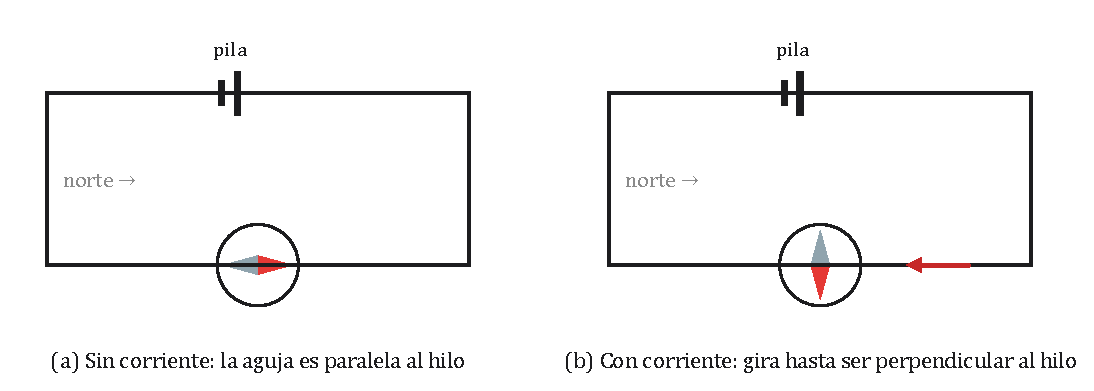
\includegraphics[width=0.9\linewidth]{images/UD6/oersted}
    \caption{Experiencia de Oersted vista desde arriba.}
    \label{fig:mag-oersted}
\end{figure}

\section{Fuerza sobre una carga en movimiento: ley de Lorentz}\label{sec:mag-lorentz}

Experimentalmente se observa que un campo magnético no ejerce fuerza sobre una carga en reposo, ni sobre una carga que se
mueve en la dirección del campo. En los demás casos la fuerza es perpendicular a la velocidad y al campo, y es máxima cuando la
carga se mueve perpendicularmente a las líneas de campo. Todo esto se resume en la \rojon{ley de Lorentz}:
\begin{centeredequation}
    \boxed{\vec F = q\,(\vec v\times\vec B)} \qquad\qquad F = |q|\,v\,B\sen\varphi \label{eq:mag-lorentz}
\end{centeredequation}
donde \(\varphi\) es el ángulo entre \(\vec v\) y \(\vec B\). El sentido de \(\vec v\times\vec B\) es el de avance de un
sacacorchos que gira llevando \(\vec v\) hacia \(\vec B\) por el camino más corto; para una carga negativa, la fuerza tiene el
sentido contrario (figura~\ref{fig:mag-lorentz}).

\begin{figure}[H]
    \centering
    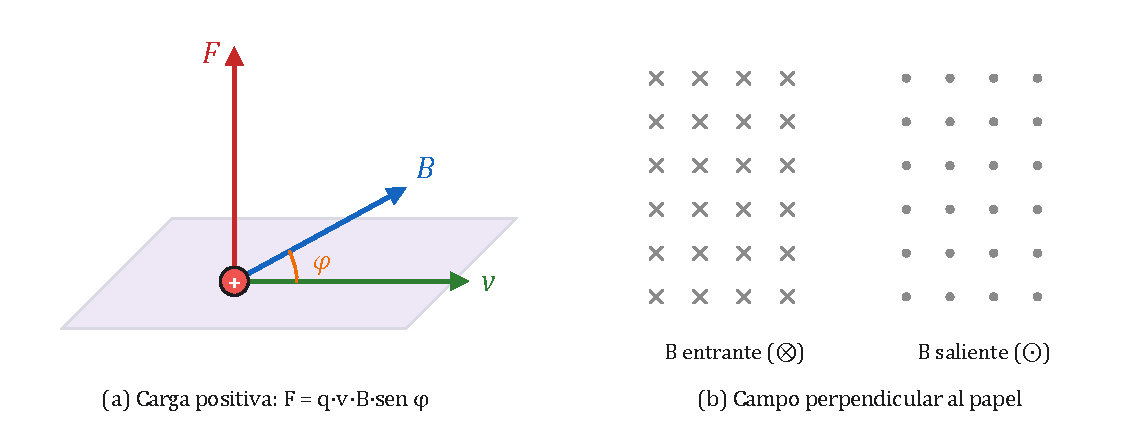
\includegraphics[width=0.9\linewidth]{images/UD6/lorentz}
    \caption{(a) La fuerza magnética es perpendicular al plano de \(\vec v\) y \(\vec B\). (b) Convenio para dibujar campos
    perpendiculares al papel: \(\times\) si entran y \(\bullet\) si salen.}
    \label{fig:mag-lorentz}
\end{figure}

\paragraph{Unidad.} La unidad de \(B\) en el SI es el \azuln{tesla} (\unit{\tesla}): el campo que ejerce una fuerza de
\qty{1}{\newton} sobre una carga de \qty{1}{\coulomb} que se mueve a \qty{1}{\m\per\second} perpendicularmente a él,
\(\qty{1}{\tesla} = \qty{1}{\newton\per\ampere\per\m}\). Es una unidad grande: el campo magnético terrestre es de unos
\qty{5e-5}{\tesla}, un imán de nevera crea unos \qty{0.01}{\tesla} y una resonancia magnética, entre \qty{1.5}{\tesla} y
\qty{3}{\tesla}.

\paragraph{Fuerza de Lorentz generalizada.} Si en una región hay a la vez un campo eléctrico y uno magnético:
\begin{centeredequation}
    \vec F = q\,\vec E + q\,(\vec v\times\vec B) = q\,(\vec E + \vec v\times\vec B) \label{eq:mag-lorentz-gen}
\end{centeredequation}

\begin{exercise}
    Una partícula con una carga de \qty{3}{\micro\coulomb} entra con una velocidad de \qty{2e6}{\m\per\second} en un campo
    magnético de \qty{2}{\tesla}, formando \ang{30} con él. ¿Qué fuerza actúa sobre ella?
    \begin{solu}
        \(F = q v B\sen\varphi = 3\cdot 10^{-6}\cdot 2\cdot 10^6\cdot 2\cdot\sen\ang{30} = \textcolor{red}{\qty{6}{\newton}}\),
        \textcolor{blue}{perpendicular al plano que forman \(\vec v\) y \(\vec B\).}
    \end{solu}
\end{exercise}

\begin{exercise}
    Un protón con una energía cinética de \qty{4}{\mega\electronvolt} se mueve perpendicularmente a un campo de \qty{1.2}{\tesla}.
    ¿Qué fuerza actúa sobre él? (\(m_p = \qty{1.67e-27}{\kg}\); \(\qty{1}{\electronvolt} = \qty{1.6e-19}{\joule}\)).
    \begin{solu}
        \(v = \sqrt{\dfrac{2E_c}{m}} = \sqrt{\dfrac{2\cdot 4\cdot 10^6\cdot 1{,}6\cdot 10^{-19}}{1{,}67\cdot 10^{-27}}} = \qty{2.77e7}{\m\per\second}\);
        \(F = q v B = \textcolor{red}{\qty{5.32e-12}{\newton}}\).
    \end{solu}
\end{exercise}

\begin{exercise}
    En una región hay un campo eléctrico \(\vec E = 2\,\vec{i} - 1000\,\vec{k}\ \unit{\newton\per\coulomb}\) y un campo magnético
    \(\vec B = 0{,}4\,\vec{i} + \vec{j}\ \unit{\tesla}\). Calcula la fuerza sobre una carga de \qty{5}{\micro\coulomb} que se mueve
    con \(\vec v = 2000\,\vec{i}\ \unit{\m\per\second}\).
    \begin{solu}
        \(\vec v\times\vec B = 2000\,\vec{i}\times(0{,}4\,\vec{i} + \vec{j}) = 2000\,\vec{k}\) \textcolor{blue}{(porque \(\vec{i}\times\vec{i} = 0\) y \(\vec{i}\times\vec{j} = \vec{k}\)).}
        \[ \vec F = q(\vec E + \vec v\times\vec B) = 5\cdot 10^{-6}\,(2\,\vec{i} + 1000\,\vec{k}) = \textcolor{red}{(1\cdot 10^{-5}\,\vec{i} + 5\cdot 10^{-3}\,\vec{k})\ \unit{\newton}} \]
    \end{solu}
\end{exercise}

\section{Movimiento de cargas en un campo magnético}\label{sec:mag-movimiento}

Como la fuerza magnética es siempre perpendicular a la velocidad, \textbf{no hace trabajo}: no cambia el módulo de la velocidad
ni la energía cinética de la partícula, solo su dirección.

\paragraph{Velocidad perpendicular al campo.} La fuerza actúa como fuerza centrípeta y la partícula describe una
\textbf{circunferencia} con movimiento uniforme (figura~\ref{fig:mag-circular}):
\begin{equation*}
    |q|\,v\,B = m\,\dfrac{v^2}{R} \qquad\Rightarrow\qquad \boxed{R = \dfrac{m\,v}{|q|\,B}}
\end{equation*}
El radio es proporcional a la cantidad de movimiento e inversamente proporcional a la carga y al campo. El período y la
frecuencia del movimiento (la \azuln{frecuencia ciclotrón}) no dependen de la velocidad ni del radio:
\begin{centeredequation}
    \omega = \dfrac{v}{R} = \dfrac{|q|\,B}{m} \qquad\qquad T = \dfrac{2\pi m}{|q|\,B} \qquad\qquad f = \dfrac{|q|\,B}{2\pi m} \label{eq:mag-ciclotron}
\end{centeredequation}
En esto se basan el \emph{ciclotrón} (un acelerador de partículas) y el \emph{espectrómetro de masas}, que separa los isótopos
de un elemento por el radio de su trayectoria.

\begin{figure}[H]
    \centering
    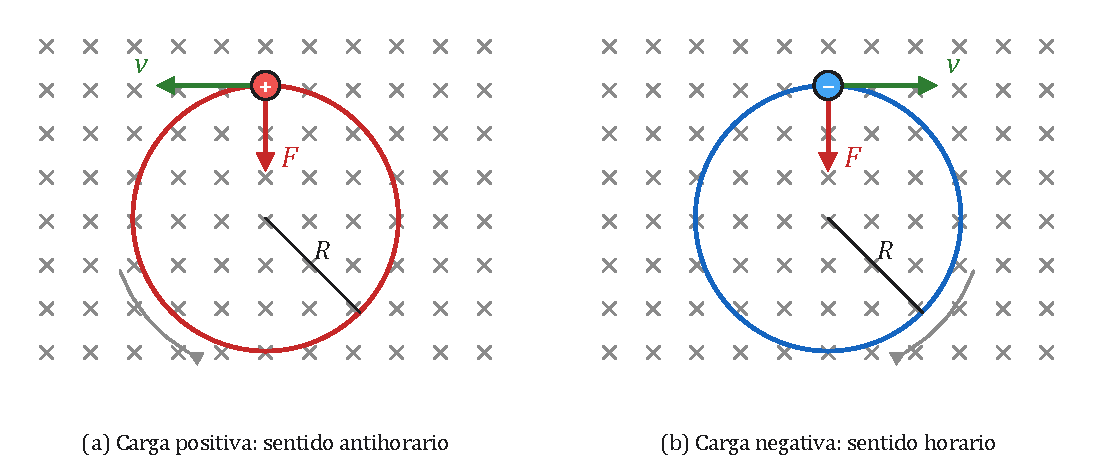
\includegraphics[width=0.9\linewidth]{images/UD6/circular}
    \caption{Trayectorias en un campo entrante: el sentido de giro depende del signo de la carga.}
    \label{fig:mag-circular}
\end{figure}

\paragraph{Velocidad oblicua.} Si la velocidad forma un ángulo con el campo, la componente paralela a \(\vec B\) no cambia y la
perpendicular produce un giro: la trayectoria es una \textbf{hélice} (figura~\ref{fig:mag-helice}). Así quedan atrapadas las
partículas del viento solar en el campo magnético terrestre; al llegar a la atmósfera cerca de los polos producen las auroras.

\begin{figure}[H]
    \centering
    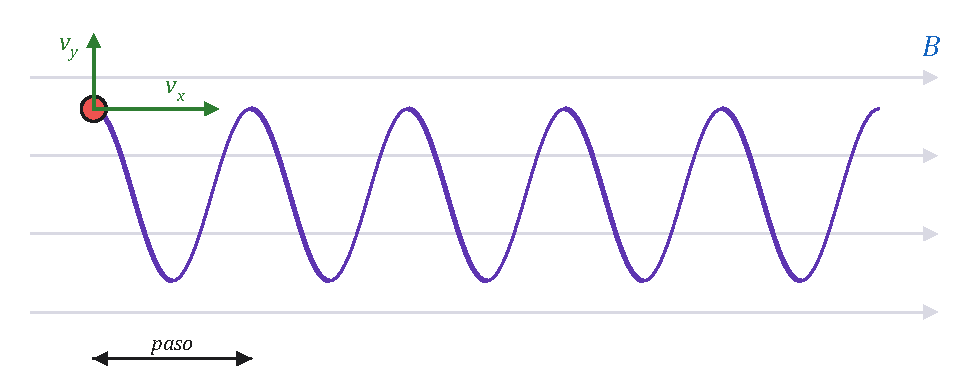
\includegraphics[width=0.66\linewidth]{images/UD6/helice}
    \caption{Trayectoria helicoidal de una carga cuya velocidad no es perpendicular al campo.}
    \label{fig:mag-helice}
\end{figure}

\begin{exercise}
    Un electrón con una velocidad de \qty{3000}{\km\per\second} entra perpendicularmente en un campo uniforme de
    \qty{2e-3}{\tesla}. Calcula el radio de su órbita y la frecuencia del movimiento (\(m_e = \qty{9.11e-31}{\kg}\)).
    \begin{solu}
        \(R = \dfrac{m v}{e B} = \dfrac{9{,}11\cdot 10^{-31}\cdot 3\cdot 10^6}{1{,}6\cdot 10^{-19}\cdot 2\cdot 10^{-3}} = \textcolor{red}{\qty{8.54e-3}{\m}}\);
        \(f = \dfrac{e B}{2\pi m} = \textcolor{red}{\qty{5.59e7}{\hertz}}\).
    \end{solu}
\end{exercise}

\begin{exercise}
    Un protón entra perpendicularmente en un campo de \qty{2}{\tesla}. ¿Con qué velocidad debe entrar para que el radio de su
    trayectoria sea de \qty{3}{\cm}?
    \begin{solu}
        \(v = \dfrac{q B R}{m} = \dfrac{1{,}6\cdot 10^{-19}\cdot 2\cdot 0{,}03}{1{,}67\cdot 10^{-27}} = \textcolor{red}{\qty{5.75e6}{\m\per\second}}\).
    \end{solu}
\end{exercise}

\section{Fuerza sobre una corriente: ley de Laplace}\label{sec:mag-laplace}

Una corriente es un conjunto de cargas en movimiento, así que un campo magnético ejerce fuerza sobre un conductor por el que
circula corriente. Si el conductor tiene \(n\) portadores de carga \(q\) por unidad de volumen, sección \(S\) y longitud \(L\), y
los portadores se mueven con velocidad \(\vec v\), la intensidad es \(I = nqSv\) y la fuerza total es
\(\vec F = nSL\,q\,(\vec v\times\vec B)\). Definiendo un vector \(\vec L\) de módulo la longitud del conductor y con el sentido de
la corriente, queda la \rojon{ley de Laplace}:
\begin{centeredequation}
    \boxed{\vec F = I\,(\vec L\times\vec B)} \qquad\qquad F = I\,L\,B\sen\alpha \label{eq:mag-laplace}
\end{centeredequation}
donde \(\alpha\) es el ángulo entre el conductor y el campo (figura~\ref{fig:mag-laplace}).

\begin{figure}[H]
    \centering
    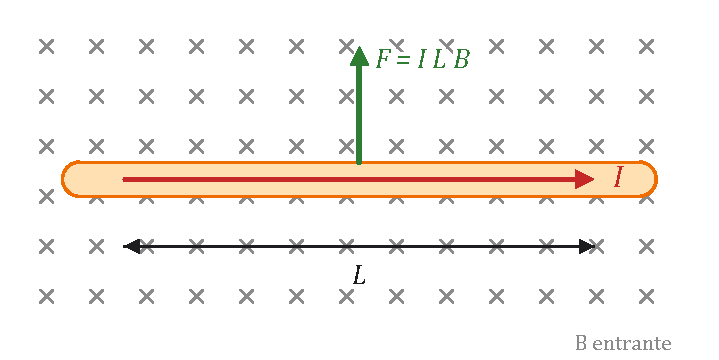
\includegraphics[width=0.55\linewidth]{images/UD6/laplace}
    \caption{Fuerza sobre un conductor perpendicular a un campo entrante.}
    \label{fig:mag-laplace}
\end{figure}

\begin{exercise}
    Un conductor de \qty{50}{\cm} por el que circula una corriente de \qty{0.4}{\ampere} está en un campo uniforme de
    \qty{0.5}{\tesla} y forma \ang{30} con él. ¿Qué fuerza actúa sobre él?
    \begin{solu}
        \(F = I L B\sen\alpha = 0{,}4\cdot 0{,}5\cdot 0{,}5\cdot\sen\ang{30} = \textcolor{red}{\qty{0.05}{\newton}}\).
    \end{solu}
\end{exercise}

\begin{exercise}
    Un conductor de \qty{20}{\cm} está sobre el eje \(Y\) y lleva una corriente de \qty{3}{\ampere} en sentido positivo. Si el
    campo es \(\vec B = 0{,}1\,\vec{i} - 0{,}2\,\vec{j} + 0{,}4\,\vec{k}\ \unit{\tesla}\), ¿qué fuerza actúa sobre él?
    \begin{solu}
        \(\vec L = 0{,}2\,\vec{j}\ \unit{\m}\).
        \(\vec L\times\vec B = 0{,}2\,\vec{j}\times(0{,}1\,\vec{i} - 0{,}2\,\vec{j} + 0{,}4\,\vec{k}) = 0{,}2\,(-0{,}1\,\vec{k} + 0{,}4\,\vec{i})\).
        \[ \vec F = I\,(\vec L\times\vec B) = \textcolor{red}{0{,}24\,\vec{i} - 0{,}06\,\vec{k}\ \unit{\newton}} \]
    \end{solu}
\end{exercise}

\subsection{Momento sobre una espira. El motor eléctrico}\label{subsec:mag-espira}

Sobre una espira rectangular de lados \(a\) y \(b\) por la que circula \(I\), en un campo uniforme, las fuerzas sobre los lados
opuestos son iguales y de sentidos contrarios. La fuerza neta es nula, pero las fuerzas sobre los dos lados perpendiculares al
campo no están en la misma recta: forman un \textbf{par de fuerzas} que hace girar la espira (figura~\ref{fig:mag-espira}). Cada
una vale \(F = I\,a\,B\) y su brazo es \(b\sen\alpha\), donde \(\alpha\) es el ángulo entre \(\vec B\) y el vector superficie
\(\vec S\) (perpendicular a la espira, con el sentido que da la regla de la mano derecha aplicada a la corriente):
\begin{centeredequation}
    M = I\,a\,B\,b\sen\alpha = I\,S\,B\sen\alpha \qquad\Rightarrow\qquad \boxed{\vec M = I\,(\vec S\times\vec B) = \vec m\times\vec B} \label{eq:mag-par}
\end{centeredequation}
El vector \(\vec m = I\vec S\) es el \azuln{momento magnético} de la espira; para una bobina de \(N\) espiras, \(\vec m = N I\vec S\).
El par tiende a girar la espira hasta que \(\vec m\) se alinea con \(\vec B\), igual que una brújula. Es el principio del
\textbf{motor eléctrico} y de los galvanómetros: si cada media vuelta se invierte el sentido de la corriente (con un colector de
delgas), el par siempre hace girar la espira en el mismo sentido.

\begin{figure}[H]
    \centering
    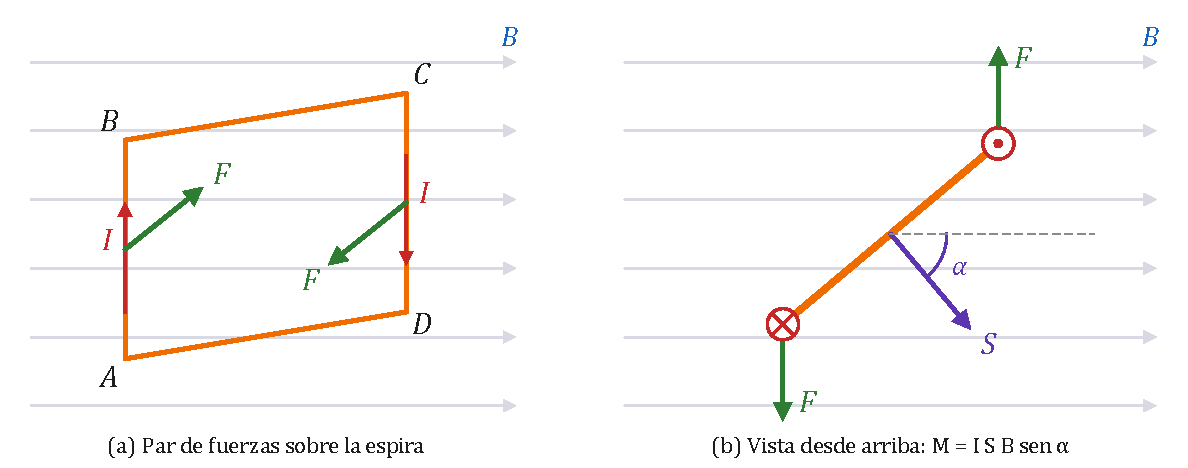
\includegraphics[width=0.95\linewidth]{images/UD6/espira_par}
    \caption{Par de fuerzas sobre una espira con corriente en un campo uniforme.}
    \label{fig:mag-espira}
\end{figure}

\begin{exercise}
    Una espira circular de \qty{12}{\cm} de diámetro, recorrida por \qty{3}{\ampere}, está en un campo de \qty{0.5}{\tesla}. Calcula
    su momento magnético y el momento del par cuando su vector superficie forma \ang{60} con el campo. ¿Cuál es el momento máximo?
    \begin{solu}
        \(S = \pi\cdot 0{,}06^2 = \qty{1.13e-2}{\m\squared}\); \(m = IS = \textcolor{red}{\qty{3.39e-2}{\ampere\m\squared}}\).

        \(M = m B\sen\ang{60} = \textcolor{red}{\qty{1.47e-2}{\newton\m}}\); \(M_{\text{máx}} = m B = \textcolor{red}{\qty{1.70e-2}{\newton\m}}\) \textcolor{blue}{(con la espira paralela al campo).}
    \end{solu}
\end{exercise}

\section{Campos magnéticos creados por corrientes}\label{sec:mag-creados}

\subsection{Campo de una carga en movimiento. Ley de Biot y Savart}\label{subsec:mag-biot}

Una carga \(q\) que se mueve con velocidad \(\vec v\) crea en un punto situado en la posición \(\vec r\) un campo:
\begin{centeredequation}
    \vec B = \dfrac{\mu_0}{4\pi}\,\dfrac{q\,\vec v\times\vec u_r}{r^2} \qquad\qquad B = \dfrac{\mu_0}{4\pi}\,\dfrac{q\,v\sen\varphi}{r^2} \label{eq:mag-carga}
\end{centeredequation}
donde \(\mu_0 = 4\pi\cdot 10^{-7}\ \unit{\tesla\m\per\ampere}\) es la \azuln{permeabilidad magnética del vacío}. Del mismo modo, un
elemento de corriente \(I\,d\vec l\) crea un campo elemental (\rojon{ley de Biot y Savart}):
\begin{centeredequation}
    d\vec B = \dfrac{\mu_0}{4\pi}\,\dfrac{I\,d\vec l\times\vec u_r}{r^2} \label{eq:mag-biot}
\end{centeredequation}
El campo de cualquier conductor se obtiene sumando (integrando) los campos de todos sus elementos.

\begin{exercise}
    En el modelo de Bohr del átomo de hidrógeno, el electrón gira alrededor del protón a \qty{5.29e-11}{\m} con una velocidad de
    \qty{2.19e6}{\m\per\second}. ¿Qué campo magnético crea en la posición del protón?
    \begin{solu}
        \textcolor{blue}{\(\vec v\) es perpendicular a \(\vec r\):}
        \(B = 10^{-7}\,\dfrac{1{,}6\cdot 10^{-19}\cdot 2{,}19\cdot 10^6}{(5{,}29\cdot 10^{-11})^2} = \textcolor{red}{\qty{12.5}{\tesla}}\):
        \textcolor{blue}{un campo enorme, a escala atómica.}
    \end{solu}
\end{exercise}

\subsection{Corriente rectilínea indefinida}\label{subsec:mag-hilo}

Integrando la ley de Biot y Savart a lo largo de un hilo infinito, a una distancia \(r\) de él:
\begin{centeredequation}
    \boxed{B = \dfrac{\mu_0\,I}{2\pi\,r}} \label{eq:mag-hilo}
\end{centeredequation}
Las líneas de campo son \textbf{circunferencias concéntricas} con el hilo, en planos perpendiculares a él. Su sentido lo da la
\azuln{regla de la mano derecha}: con el pulgar en el sentido de la corriente, los demás dedos se cierran en el sentido del campo
(figura~\ref{fig:mag-hilo}).

\begin{figure}[H]
    \centering
    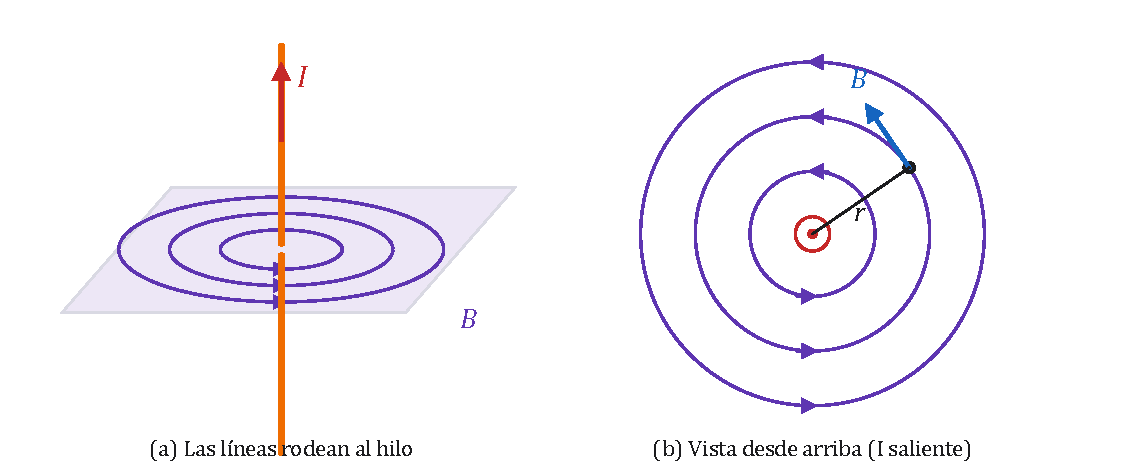
\includegraphics[width=0.92\linewidth]{images/UD6/hilo}
    \caption{Campo de una corriente rectilínea. \(\vec B\) es tangente a las circunferencias.}
    \label{fig:mag-hilo}
\end{figure}

\begin{exercise}
    Dos conductores perpendiculares al papel, separados \qty{30}{\cm}, llevan corrientes de \qty{6}{\ampere} y \qty{10}{\ampere}
    entrantes. Calcula el campo en el punto medio. ¿En qué punto de la recta que los une se anula?
    \begin{solu}
        \textcolor{blue}{En el punto medio los dos campos tienen sentidos opuestos:}
        \(B = \dfrac{\mu_0}{2\pi}\,\dfrac{10 - 6}{0{,}15} = \textcolor{red}{\qty{5.33e-6}{\tesla}}\), \textcolor{blue}{en el sentido del creado por el de \qty{10}{\ampere}.}

        \textcolor{blue}{Se anula entre ellos, a una distancia \(x\) del de \qty{6}{\ampere}:} \(\dfrac{6}{x} = \dfrac{10}{0{,}3 - x} \Rightarrow \textcolor{red}{x = \qty{11.25}{\cm}}\).
    \end{solu}
\end{exercise}

\subsection{Espira circular}\label{subsec:mag-espira-circular}

En el centro de una espira de radio \(R\), todos los elementos de corriente son perpendiculares al radio y están a la misma
distancia, así que sus campos se suman directamente:
\begin{centeredequation}
    B = \dfrac{\mu_0 I}{4\pi R^2}\oint dl = \dfrac{\mu_0 I}{4\pi R^2}\,2\pi R \qquad\Rightarrow\qquad \boxed{B = \dfrac{\mu_0\,I}{2R}} \label{eq:mag-espira}
\end{centeredequation}
El campo es perpendicular al plano de la espira, con el sentido que da la regla de la mano derecha (figura~\ref{fig:mag-espira-campo}).
Para una bobina plana de \(N\) espiras, \(B = N\mu_0 I/2R\). Una espira se comporta como un imán: la cara por la que salen las
líneas es un polo norte.

\begin{figure}[H]
    \centering
    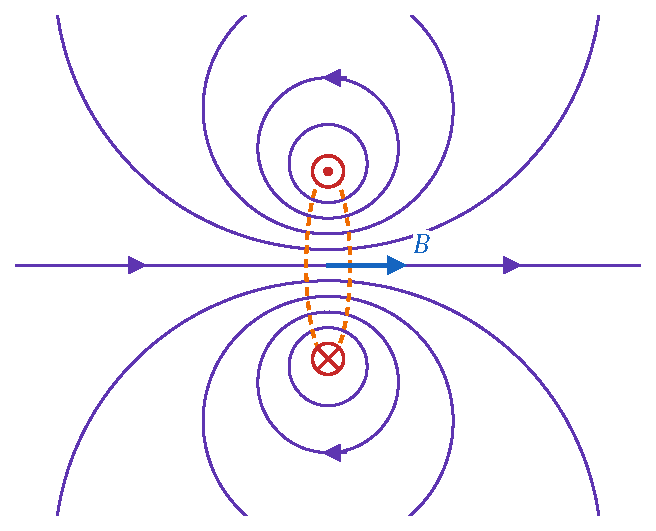
\includegraphics[width=0.45\linewidth]{images/UD6/espira_campo}
    \caption{Líneas del campo de una espira circular en un corte por su eje.}
    \label{fig:mag-espira-campo}
\end{figure}

\begin{exercise}
    ¿Qué radio tiene una espira por la que circulan \qty{4}{\ampere} si el campo en su centro es de \qty{2e-5}{\tesla}?
    \begin{solu}
        \(R = \dfrac{\mu_0 I}{2B} = \dfrac{4\pi\cdot 10^{-7}\cdot 4}{2\cdot 2\cdot 10^{-5}} = \textcolor{red}{\qty{0.126}{\m}}\).
    \end{solu}
\end{exercise}

\subsection{Ley de Ampère}\label{subsec:mag-ampere}

En los campos gravitatorio y eléctrico la \emph{circulación} del campo a lo largo de una línea cerrada es nula: son campos
conservativos. Para el campo magnético no ocurre lo mismo. Calculemos la circulación a lo largo de una circunferencia de
radio \(r\) centrada en un hilo: \(\vec B\) y \(d\vec l\) son paralelos y \(B\) es constante,
\begin{equation*}
    \oint\vec B\cdot d\vec l = B\oint dl = \dfrac{\mu_0 I}{2\pi r}\,2\pi r = \mu_0 I
\end{equation*}

\begin{definition}[Ley de Ampère]
    La circulación del campo magnético a lo largo de cualquier línea cerrada es igual a \(\mu_0\) por la intensidad neta que
    atraviesa la superficie limitada por esa línea:
    \begin{centeredequation}
        \boxed{\oint\vec B\cdot d\vec l = \mu_0\sum I} \label{eq:mag-ampere}
    \end{centeredequation}
    Se cuentan como positivas las corrientes cuyo sentido coincide con el que da la regla de la mano derecha al recorrer la línea.
\end{definition}

Como la circulación no es nula, \textbf{el campo magnético no es conservativo}: no se puede definir un potencial magnético como
en los otros campos.

\paragraph{Campo de un solenoide.} Un \rojon{solenoide} es un conjunto de espiras iguales enrolladas en hélice, con una longitud
\(L\) mucho mayor que su radio. Dentro, el campo es prácticamente uniforme y paralelo al eje; fuera, casi nulo (salvo cerca de
los extremos, donde se parece al de un imán de barra). Aplicando la ley de Ampère al rectángulo \(ACDE\) de la
figura~\ref{fig:mag-solenoide}: en los lados \(CD\) y \(EA\) el campo es perpendicular al camino; en \(DE\), fuera, es nulo; solo
contribuye el lado \(AC\), de longitud \(l\), por dentro. Si hay \(n = N/L\) espiras por unidad de longitud, el rectángulo encierra
\(n\,l\) espiras:
\begin{equation*}
    B\,l = \mu_0\,n\,l\,I \qquad\Rightarrow\qquad \boxed{B = \mu_0\,\dfrac{N}{L}\,I = \mu_0\,n\,I}
\end{equation*}

\begin{figure}[H]
    \centering
    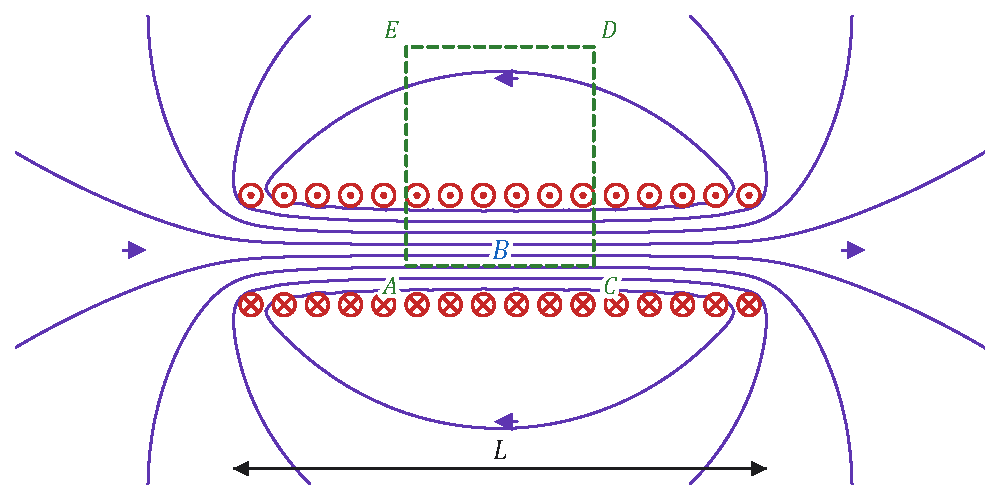
\includegraphics[width=0.75\linewidth]{images/UD6/solenoide}
    \caption{Corte de un solenoide (líneas de campo calculadas) y camino rectangular para aplicar la ley de Ampère.}
    \label{fig:mag-solenoide}
\end{figure}

Si el solenoide se enrolla sobre un núcleo de hierro, el campo se multiplica cientos de veces: es un \textbf{electroimán}.

\begin{exercise}
    ¿Qué longitud debe tener un solenoide de 800 espiras, por el que circulan \qty{1.5}{\ampere}, para que el campo en su interior
    sea de \qty{6e-3}{\tesla}?
    \begin{solu}
        \(L = \dfrac{\mu_0 N I}{B} = \dfrac{4\pi\cdot 10^{-7}\cdot 800\cdot 1{,}5}{6\cdot 10^{-3}} = \textcolor{red}{\qty{0.251}{\m}}\).
    \end{solu}
\end{exercise}

\subsection{Fuerzas entre corrientes paralelas}\label{subsec:mag-paralelas}

Dos conductores rectilíneos y paralelos, separados \(d\), se ejercen fuerzas: el campo que crea el primero en la posición del
segundo, \(B_1 = \mu_0 I_1/2\pi d\), actúa sobre la corriente \(I_2\) según la ley de Laplace, y al revés:
\begin{centeredequation}
    \boxed{\dfrac{F}{L} = \dfrac{\mu_0\,I_1\,I_2}{2\pi\,d}} \label{eq:mag-paralelas}
\end{centeredequation}
\textbf{Las corrientes del mismo sentido se atraen y las de sentidos opuestos se repelen} (figura~\ref{fig:mag-paralelas}): justo
al revés que las cargas.

\begin{figure}[H]
    \centering
    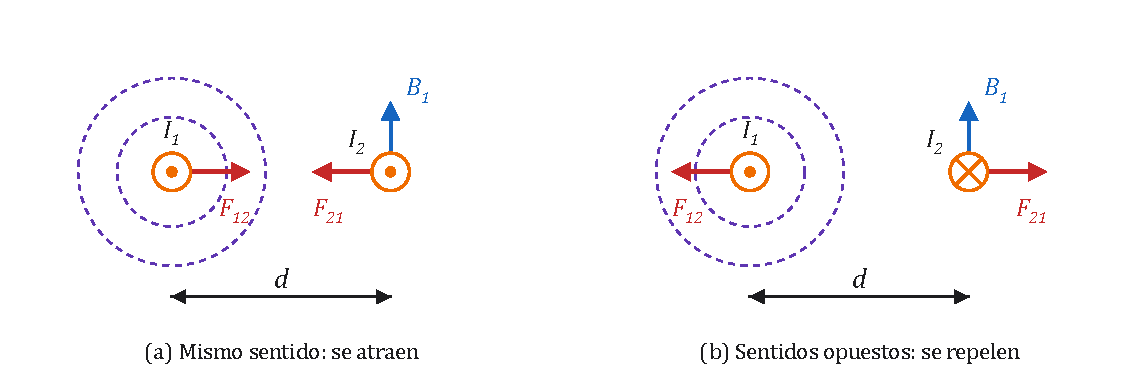
\includegraphics[width=0.9\linewidth]{images/UD6/paralelas}
    \caption{Fuerzas entre dos corrientes paralelas, vistas en corte.}
    \label{fig:mag-paralelas}
\end{figure}

\begin{remark}
    Esta fuerza sirvió para definir el \textbf{amperio}: la corriente que, circulando por dos conductores paralelos, rectilíneos e
    indefinidos, separados \qty{1}{\m} en el vacío, hace que se atraigan con una fuerza de \qty{2e-7}{\newton} por metro. (Desde
    2019 el amperio se define a partir del valor fijo de la carga del electrón, pero la relación sigue siendo válida.)
\end{remark}

\begin{exercise}
    Dos hilos paralelos de \qty{30}{\cm} están separados \qty{20}{\cm} y llevan \qty{40}{\ampere} cada uno en el mismo sentido.
    ¿Qué fuerza se ejercen?
    \begin{solu}
        \(F = \dfrac{\mu_0 I_1 I_2 L}{2\pi d} = 2\cdot 10^{-7}\,\dfrac{40\cdot 40\cdot 0{,}3}{0{,}2} = \textcolor{red}{\qty{4.8e-4}{\newton}}\), \textcolor{red}{de atracción}.
    \end{solu}
\end{exercise}

\section{Inducción electromagnética}\label{sec:mag-induccion}

\subsection{Flujo magnético}\label{subsec:mag-flujo}

El \rojon{flujo magnético} a través de una superficie mide el número de líneas de campo que la atraviesan. Para un campo
uniforme y una superficie plana:
\begin{centeredequation}
    \boxed{\Phi = \vec B\cdot\vec S = B\,S\cos\alpha} \label{eq:mag-flujo}
\end{centeredequation}
donde \(\alpha\) es el ángulo entre \(\vec B\) y el vector superficie. En general, \(\Phi = \int\vec B\cdot d\vec S\). Su unidad es
el \azuln{weber}: \(\qty{1}{\weber} = \qty{1}{\tesla\m\squared}\). Como las líneas del campo magnético son cerradas, todas las que
entran en una superficie cerrada salen de ella: \textbf{el flujo magnético a través de una superficie cerrada es siempre nulo}
(no hay polos magnéticos aislados).

\begin{exercise}
    Calcula el flujo magnético a través de una espira cuadrada de \qty{10}{\cm} de lado perpendicular a un campo de
    \qty{0.8}{\tesla}, y a través de una espira circular de \qty{30}{\cm} de diámetro cuyo eje forma \ang{60} con un campo de
    \qty{0.5}{\tesla}.
    \begin{solu}
        \(\Phi_1 = B S = 0{,}8\cdot 0{,}01 = \textcolor{red}{\qty{8e-3}{\weber}}\);
        \(\Phi_2 = B S\cos\ang{60} = 0{,}5\cdot\pi\cdot 0{,}15^2\cdot 0{,}5 = \textcolor{red}{\qty{1.77e-2}{\weber}}\).
    \end{solu}
\end{exercise}

\subsection{Experiencias de Faraday y Henry}\label{subsec:mag-faraday}

Faraday conectó una bobina a un galvanómetro (un amperímetro muy sensible) y observó (figura~\ref{fig:mag-faraday}):
\begin{itemize}
    \item al acercar un imán, el galvanómetro marca corriente, y más cuanto más deprisa se mueve el imán;
    \item si el imán se para, la corriente cesa;
    \item al alejarlo, la corriente circula en sentido contrario; lo mismo ocurre si se acerca el otro polo;
    \item se obtiene lo mismo dejando quieto el imán y moviendo la bobina, o cambiando la corriente de otra bobina cercana.
\end{itemize}
A la corriente que aparece se le llama \azuln{corriente inducida}, y a la fuerza electromotriz que la produce, \azuln{fem inducida}.
El circuito donde aparece es el \emph{inducido} y el agente que la produce (el imán), el \emph{inductor}.

\begin{figure}[H]
    \centering
    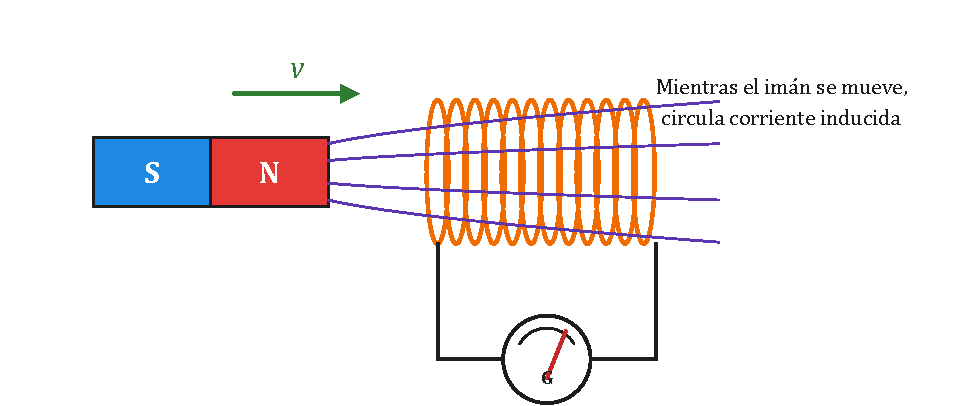
\includegraphics[width=0.7\linewidth]{images/UD6/faraday}
    \caption{Experiencia de Faraday.}
    \label{fig:mag-faraday}
\end{figure}

Henry, por su parte, observó que un conductor que se mueve cortando las líneas de un campo magnético tiene una diferencia de
potencial entre sus extremos. Sobre los electrones del conductor actúa la fuerza de Lorentz, que los acumula en un extremo. Si una
varilla de longitud \(l\) se mueve con velocidad \(v\) perpendicular a \(B\) (figura~\ref{fig:mag-varilla}), el trabajo por unidad
de carga a lo largo de la varilla es la fem:
\begin{centeredequation}
    \varepsilon = \dfrac{F\,l}{q} = \dfrac{q\,v\,B\,l}{q} \qquad\Rightarrow\qquad \boxed{\varepsilon = B\,l\,v} \label{eq:mag-Blv}
\end{centeredequation}
Si la varilla cierra un circuito, circula corriente; entonces el campo ejerce sobre la varilla una fuerza (ley de Laplace) que se
opone al movimiento, y hay que empujarla para mantener la velocidad: así se transforma energía mecánica en eléctrica.

\begin{figure}[H]
    \centering
    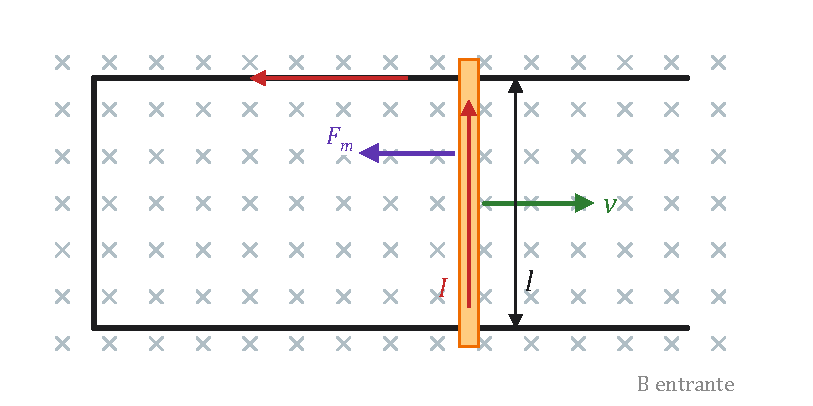
\includegraphics[width=0.6\linewidth]{images/UD6/varilla}
    \caption{Varilla que se desliza sobre unos raíles en un campo entrante.}
    \label{fig:mag-varilla}
\end{figure}

\subsection{Ley de Faraday-Lenz}\label{subsec:mag-faraday-lenz}

Todas estas experiencias tienen algo en común: \textbf{varía el flujo magnético} a través del circuito (por moverse el imán,
cambiar el área o la orientación del circuito, o cambiar el campo).

\begin{definition}[Ley de Faraday-Lenz]
    La fem inducida en un circuito es igual a la rapidez con que varía el flujo magnético que lo atraviesa, cambiada de signo.
    Para una bobina de \(N\) espiras:
    \begin{centeredequation}
        \boxed{\varepsilon = -N\,\dfrac{d\Phi}{dt}} \qquad\qquad \varepsilon_{\text{media}} = -N\,\dfrac{\Delta\Phi}{\Delta t} \label{eq:mag-faraday}
    \end{centeredequation}
\end{definition}

El signo menos expresa la \rojon{ley de Lenz}: \emph{la corriente inducida circula en el sentido en que su propio campo magnético
se opone a la variación del flujo que la produce}. Si el flujo aumenta, el campo inducido es contrario al inductor; si disminuye,
tiene su mismo sentido. Es una consecuencia de la conservación de la energía: si la corriente inducida favoreciera el cambio, se
crearía energía de la nada.

\begin{figure}[H]
    \centering
    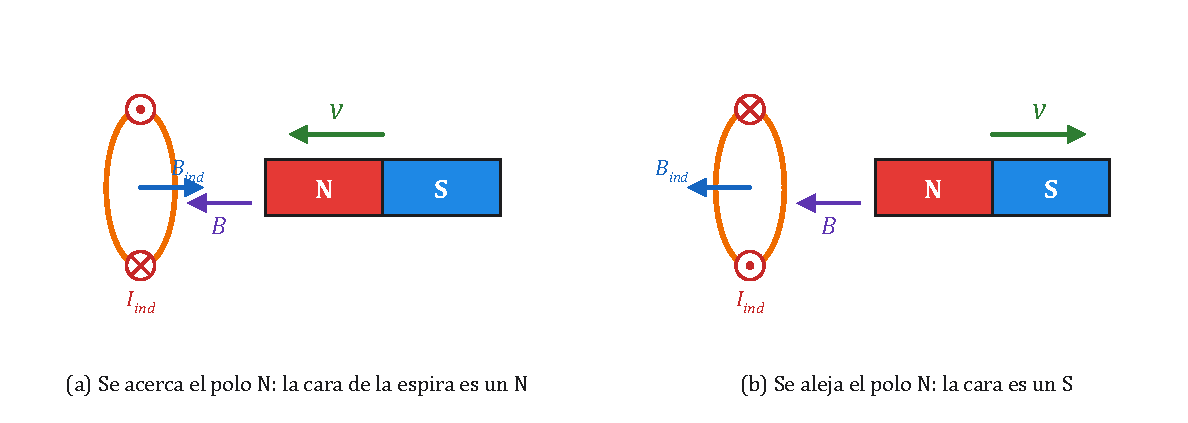
\includegraphics[width=0.95\linewidth]{images/UD6/lenz}
    \caption{Ley de Lenz. (a) Al acercar el polo norte, la espira crea un polo norte enfrente que lo repele. (b) Al alejarlo,
    crea un polo sur que lo atrae. En los dos casos la espira se opone al movimiento del imán.}
    \label{fig:mag-lenz}
\end{figure}

Con la varilla de la figura~\ref{fig:mag-varilla} se comprueba que las dos leyes coinciden: el área del circuito aumenta
\(dS = l\,v\,dt\), el flujo aumenta \(d\Phi = B\,l\,v\,dt\) y \(|\varepsilon| = d\Phi/dt = Blv\). Como el flujo entrante aumenta, la
corriente circula en sentido antihorario, creando un campo saliente.

\begin{exercise}
    Una bobina de 400 espiras cuadradas de \qty{5}{\cm} de lado está perpendicular a un campo que pasa de \qty{0.3}{\tesla} a
    \qty{0.8}{\tesla} en \qty{0.02}{\second}. ¿Qué fem media se induce?
    \begin{solu}
        \(|\varepsilon| = N S\,\dfrac{\Delta B}{\Delta t} = 400\cdot 0{,}0025\cdot\dfrac{0{,}5}{0{,}02} = \textcolor{red}{\qty{25}{\volt}}\).
    \end{solu}
\end{exercise}

\begin{exercise}
    Una varilla de \qty{40}{\cm} se mueve a \qty{5}{\m\per\second} sobre unos raíles, perpendicular a un campo de \qty{0.3}{\tesla}.
    Calcula la fem inducida y, si la resistencia del circuito es de \qty{2}{\ohm}, la intensidad y la fuerza que hay que hacer para
    mantener la velocidad.
    \begin{solu}
        \(\varepsilon = Blv = 0{,}3\cdot 0{,}4\cdot 5 = \textcolor{red}{\qty{0.6}{\volt}}\); \(I = \dfrac{\varepsilon}{R} = \textcolor{red}{\qty{0.3}{\ampere}}\);
        \(F = I l B = 0{,}3\cdot 0{,}4\cdot 0{,}3 = \textcolor{red}{\qty{0.036}{\newton}}\) \textcolor{blue}{(igual a la fuerza magnética que lo frena).}
    \end{solu}
\end{exercise}

\section{Aplicaciones de la inducción}\label{sec:mag-aplicaciones}

\subsection{El alternador}\label{subsec:mag-alternador}

Una bobina de \(N\) espiras de área \(S\) gira con velocidad angular constante \(\omega\) en un campo uniforme \(B\)
(figura~\ref{fig:mag-alternador}). El ángulo entre \(\vec B\) y \(\vec S\) es \(\alpha = \omega t\), y el flujo,
\(\Phi = B S\cos\omega t\). Por la ley de Faraday:
\begin{centeredequation}
    \varepsilon = -N\,\dfrac{d\Phi}{dt} = N B S\omega\sen\omega t \qquad\Rightarrow\qquad \boxed{\varepsilon = \varepsilon_0\sen\omega t,\quad \varepsilon_0 = N B S\omega} \label{eq:mag-alternador}
\end{centeredequation}
La fem es sinusoidal y la corriente cambia de sentido periódicamente: es una \textbf{corriente alterna}. Los extremos de la bobina
se conectan a unos anillos colectores sobre los que rozan unas escobillas, que llevan la corriente al circuito exterior. Si en
lugar de dos anillos se usa un anillo partido en dos mitades (conmutador), la corriente sale siempre en el mismo sentido: es una
\emph{dinamo}. El alternador transforma energía mecánica en eléctrica; el motor hace lo contrario.

\begin{figure}[H]
    \centering
    \begin{minipage}[b]{0.52\linewidth}
        \centering
        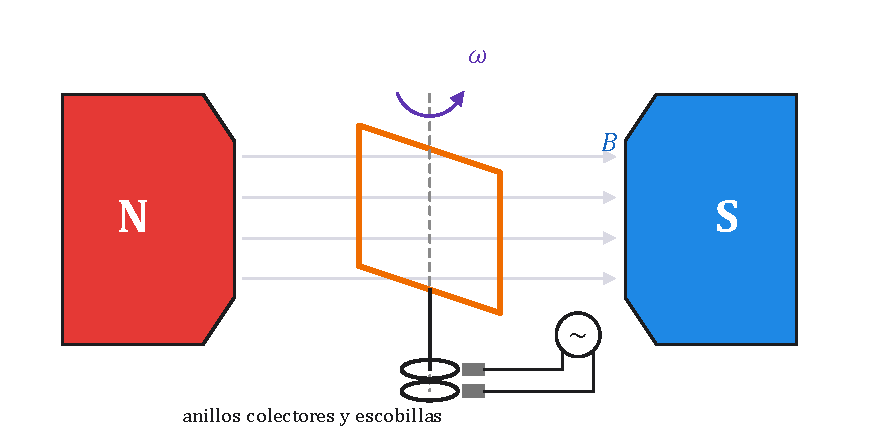
\includegraphics[width=\linewidth]{images/UD6/alternador}
    \end{minipage}\hfill
    \begin{minipage}[b]{0.44\linewidth}
        \centering
        \begin{tikzpicture}
            \begin{axis}[fisica, width=\linewidth, height=4.4cm, xmin=0, xmax=2.3, ymin=-1.35, ymax=1.45,
                xlabel={\(t\)}, ylabel={\(\varepsilon\)}, xtick={0.5,1,1.5,2}, xticklabels={\(\frac{T}{4}\),\(\frac{T}{2}\),\(\frac{3T}{4}\),\(T\)},
                ytick={-1,1}, yticklabels={\(-\varepsilon_0\),\(\varepsilon_0\)}]
                \addplot[domain=0:2.15, very thick, ocre, samples=120] {sin(deg(pi*x))};
            \end{axis}
        \end{tikzpicture}
    \end{minipage}
    \caption{Alternador y fem alterna que produce.}
    \label{fig:mag-alternador}
\end{figure}

\begin{exercise}
    Un alternador tiene una bobina de 200 espiras de \qty{100}{\cm\squared} que gira a \qty{50}{\hertz} en un campo de
    \qty{0.4}{\tesla}. ¿Cuál es la fem máxima? Escribe la expresión de la fem en función del tiempo.
    \begin{solu}
        \(\omega = 2\pi\cdot 50 = 100\pi\ \unit{\radian\per\second}\); \(\varepsilon_0 = N B S\omega = 200\cdot 0{,}4\cdot 0{,}01\cdot 100\pi = \textcolor{red}{\qty{251}{\volt}}\).
        \[ \textcolor{red}{\varepsilon = 251\sen(100\pi t)\ \text{(V)}} \]
    \end{solu}
\end{exercise}

\subsection{El transformador}\label{subsec:mag-transformador}

Un \rojon{transformador} cambia la tensión de una corriente alterna. Tiene dos bobinas enrolladas en un mismo núcleo de hierro: el
\emph{primario}, de \(N_1\) espiras, conectado a la tensión alterna \(V_1\), y el \emph{secundario}, de \(N_2\) espiras
(figura~\ref{fig:mag-transformador}). El núcleo conduce el flujo variable del primario hasta el secundario, de modo que el flujo
por espira es el mismo en las dos. Por la ley de Faraday:
\begin{equation*}
    V_1 = -N_1\,\dfrac{d\Phi}{dt} \qquad V_2 = -N_2\,\dfrac{d\Phi}{dt} \qquad\Rightarrow\qquad \boxed{\dfrac{V_2}{V_1} = \dfrac{N_2}{N_1}}
\end{equation*}
Si \(N_2 > N_1\) el transformador es \emph{elevador}; si \(N_2 < N_1\), \emph{reductor}. En un transformador ideal la potencia se
conserva, \(V_1 I_1 = V_2 I_2\), así que las intensidades están en razón inversa a las tensiones: \(I_2/I_1 = N_1/N_2\).

\begin{figure}[H]
    \centering
    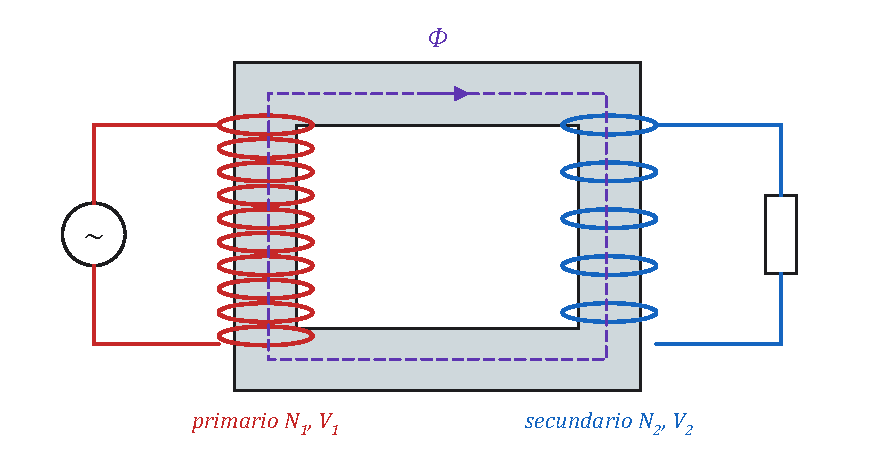
\includegraphics[width=0.6\linewidth]{images/UD6/transformador}
    \caption{Transformador reductor.}
    \label{fig:mag-transformador}
\end{figure}

\begin{remark}
    La energía eléctrica se transporta a muy alta tensión (cientos de miles de voltios) porque, para la misma potencia, la
    intensidad es menor y se pierde menos energía por efecto Joule en los cables (\(P_{\text{perdida}} = I^2 R\)). Junto a las
    centrales hay transformadores elevadores, y cerca de las ciudades, reductores. Los transformadores solo funcionan con corriente
    alterna: con corriente continua el flujo no varía.
\end{remark}

\begin{exercise}
    Un transformador tiene 1100 espiras en el primario, conectado a \qty{220}{\volt}, y 60 en el secundario. ¿Qué tensión da? Si
    por el secundario circulan \qty{2}{\ampere}, ¿qué intensidad circula por el primario?
    \begin{solu}
        \(V_2 = V_1\,\dfrac{N_2}{N_1} = \textcolor{red}{\qty{12}{\volt}}\); \(I_1 = I_2\,\dfrac{V_2}{V_1} = \textcolor{red}{\qty{0.109}{\ampere}}\).
    \end{solu}
\end{exercise}

\section{Resumen de fórmulas}\label{sec:mag-resumen}

\begin{table}[H]
    \centering
    \caption{Fórmulas principales del campo magnético y la inducción}
    \vspace{-5pt}
    \begin{tabular}{@{}lL{10cm}@{}}
        \toprule
        \textbf{Magnitud} & \textbf{Expresión} \\
        \midrule
        Ley de Lorentz & \(\vec F = q(\vec v\times\vec B)\), \quad \(F = |q| v B\sen\varphi\); \quad con \(\vec E\): \(\vec F = q(\vec E + \vec v\times\vec B)\) \\[3pt]
        Movimiento circular & \(R = m v/(|q| B)\), \quad \(T = 2\pi m/(|q| B)\) \\[3pt]
        Ley de Laplace & \(\vec F = I(\vec L\times\vec B)\), \quad \(F = I L B\sen\alpha\) \\[3pt]
        Espira en un campo & \(\vec M = \vec m\times\vec B\), \quad \(\vec m = N I\vec S\) \\[3pt]
        Hilo, espira, solenoide & \(B = \mu_0 I/(2\pi r)\); \quad \(B = \mu_0 I/(2R)\); \quad \(B = \mu_0 N I/L\) \\[3pt]
        Ley de Ampère & \(\oint\vec B\cdot d\vec l = \mu_0\sum I\), \quad \(\mu_0 = 4\pi\cdot 10^{-7}\ \unit{\tesla\m\per\ampere}\) \\[3pt]
        Corrientes paralelas & \(F/L = \mu_0 I_1 I_2/(2\pi d)\) \\[3pt]
        Flujo magnético & \(\Phi = \vec B\cdot\vec S = B S\cos\alpha\) \quad (\unit{\weber}) \\[3pt]
        Faraday-Lenz & \(\varepsilon = -N\,d\Phi/dt\); \quad varilla: \(\varepsilon = B l v\) \\[3pt]
        Alternador & \(\varepsilon = N B S\omega\sen\omega t\) \\[3pt]
        Transformador & \(V_2/V_1 = N_2/N_1 = I_1/I_2\) \\
        \bottomrule
    \end{tabular}
    \label{tab:mag-resumen}
\end{table}

\section{Prácticas de laboratorio}\label{sec:mag-practicas}

\subsection{Práctica 1: inducción electromagnética}\label{subsec:mag-practica-induccion}

\textbf{Objetivo.} Reproducir las experiencias de Faraday y comprobar la ley de Lenz.

\textbf{Material.} Bobina de muchas espiras (o dos bobinas y un núcleo de hierro), imán de barra, galvanómetro de cero central (o
un microamperímetro), pila y cables. Si no hay galvanómetro, sirve un osciloscopio o un sensor de tensión conectado al ordenador.

\textbf{Procedimiento.}
\begin{enumerate}[label=\numberballmDarkTeal]
    \item Conecta la bobina al galvanómetro (figura~\ref{fig:mag-faraday}). Introduce el polo norte del imán y anota hacia dónde se
    desvía la aguja. Déjalo quieto dentro y sácalo.
    \item Repite moviendo el imán más deprisa y con el polo sur. Repite dejando el imán fijo y moviendo la bobina.
    \item Coloca una segunda bobina conectada a la pila junto a la primera. Observa el galvanómetro al cerrar el circuito, mientras
    está cerrado y al abrirlo.
\end{enumerate}

\textbf{Cuestiones.}
\begin{enumerate}[label=\letraminuscula]
    \item ¿En qué casos hay corriente inducida? ¿Qué tienen en común?
    \item ¿De qué depende el valor de la desviación? ¿Y su sentido?
    \item Con la regla de la mano derecha, deduce qué polo forma la cara de la bobina que mira al imán cuando lo acercas y cuando lo
    alejas. Comprueba que se cumple la ley de Lenz.
\end{enumerate}

\subsection{Práctica 2: medida del campo magnético terrestre}\label{subsec:mag-practica-tangentes}

\noindent\begin{minipage}[t]{0.6\linewidth}
\textbf{Objetivo.} Medir la componente horizontal del campo magnético de la Tierra con una brújula de tangentes.

\textbf{Material.} Bobina plana de \(N\) espiras y radio \(R\) conocidos (por ejemplo, 10 espiras de \qty{10}{\cm}), brújula,
fuente de corriente continua regulable, amperímetro y reóstato.

\textbf{Procedimiento.}
\begin{enumerate}[label=\numberballmDarkTeal]
    \item Pon la brújula en el centro de la bobina y gira esta hasta que su plano contenga a la aguja (dirección norte-sur)
    (figura~\ref{fig:mag-practica}).
    \item Haz pasar corriente y mide el ángulo \(\varphi\) que gira la aguja para varias intensidades.
\end{enumerate}
\end{minipage}\hfill
\begin{minipage}[t]{0.36\linewidth}
    \vspace{0pt}
    \centering
    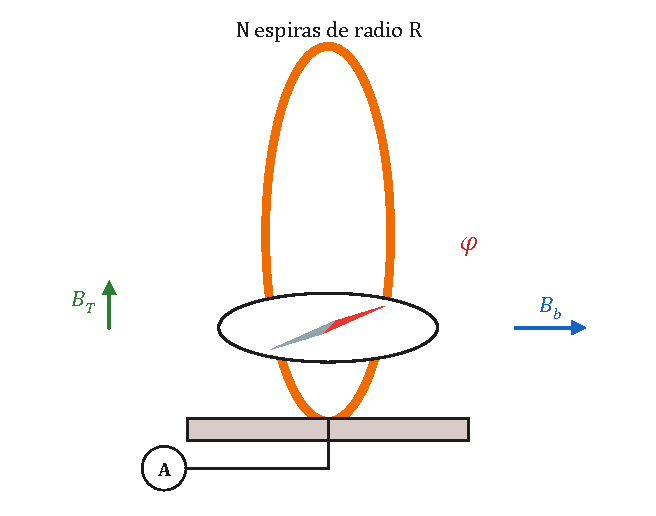
\includegraphics[width=\linewidth]{images/UD6/practica_bobina}
    \captionof{figure}{Brújula de tangentes.}
    \label{fig:mag-practica}
\end{minipage}

\textbf{Fundamento y cálculos.} La aguja se orienta según la suma del campo terrestre \(B_T\) (norte-sur) y el de la bobina,
\(B_b = N\mu_0 I/2R\), perpendicular a él. Por tanto \(\tg\varphi = B_b/B_T\). Representa \(\tg\varphi\) frente a \(I\): sale una
recta de pendiente \(N\mu_0/(2R B_T)\), de la que se obtiene \(B_T\).

\textbf{Cuestiones.}
\begin{enumerate}[label=\letraminuscula]
    \item Compara tu resultado con el valor de la componente horizontal en España (unos \qty{2.5e-5}{\tesla}).
    \item ¿Por qué hay que alejar la experiencia de objetos de hierro y de otros cables con corriente?
    \item ¿Qué ocurre si inviertes el sentido de la corriente?
\end{enumerate}
